\chapter{Decentralised Vehicle Allocation for SEC-Based Ride-Sharing Services}
\label{chapter4}
Rapid urbanisation presents environmental and logistical difficulties \cite{Reference151}. This is particularly the case for rapidly growing cities, which are prone to dynamic urban environments and fluctuating travel demands \cite{Reference3020}. In such a context, the proliferation of SECs within the city presents a decentralised alternative to the traditional central management from the city authority, as each SEC can be independently in charge of managing its own AEV fleet and demands (TP requests from its neighbours).
Conventional ride-sharing systems typically fail to capture the complex dynamics of ride-sharing networks due to centralised optimisation methodologies \cite{Reference1,Reference2,Reference4,Reference6}. For the ride-sharing model presented in Chapter 3 to truly become applicable to large-scale cities, it must apply a decentralised approach enabling it to capture the complex dynamics among the different SECs placed in the city, their energy production and the ability of their AEV fleets to serve TPs. 

This chapter addresses such a problem by extending the ride-sharing model of Chapter 3, which focused solely on the formulation, solution approach and evaluation of the reactive ride-sharing service. A new model is designed, implemented and evaluated; its main goal is to capture the interrelation among the different SECs in the city as they compete for the allocation of the AEV fleet. The process is modelled as a decentralised negotiation process, deciding the number of AEVs allocated to each SEC. The new model works in tandem with the ride-sharing model of Chapter \ref{chapter3}; given its output (i.e., the partition of the AEV fleet among the SECs), each SEC then uses the ride-sharing model of Chapter 3 to serve the TPs of its own neighbouring SECs.

Specifically, the chapter includes the following contributions:

\begin{enumerate}
    \item The formulation of the vehicle allocation problem both as a centralised optimisation problem (using a
    Mixed-Integer Programming formulation) and as a decentralised one, using an iterative negotiation process
    among connected-SECs. On the latter, each SEC acts as an independent agent, and
    carries out a number of negotiations with any other SEC it is connected to over a simulated time horizon.
    In such negotiations, connected SECs decide the potential exchange of AEVs among them, based solely on their
    local information. The criticality of the vehicle allocation problem lies on its cooperation with its underlying ride-sharing problem to ensure adequate vehicle-to-passenger matching.
    Once assigned a fixed number of vehicles, the problem of each SEC operating its own ride-sharing service is solved using the ride-sharing model presented in Chapter \ref{chapter3}.
    
    \item The implementation of the vehicle allocation problem, using a novel Multi-Objective and Multi-Agent
    Reinforcement Learning (RL) algorithm, involving Deep Q-Learning with Graph Convolutional Networks. The algorithm
    equips SECs with the ability to learn from previous-negotiations,
    enabling them to improve their decision-making as the simulated time horizon goes by \cite{Reference103}.
    
    \item The evaluation of the solution approach for the problem tandem, measuring the performance of the solution approach under different SEC connectivity-levels
    and transport request distributions, when applied to the Google HashCode and NYC aligned datasets as described in Chapter 3. .
\end{enumerate}

The structure of the chapter is as follows:
\begin{itemize}
  \item \textbf{Section~\ref{sec:ccis_problem}} explains the vehicle‑allocation problem.
  \item \textbf{Section~\ref{ccis_reinforcement_learning_solution_approach}} describes how we solve it.
  \item \textbf{Section~\ref{sec:evaluation}} shows how we tested the solution.
  \item \textbf{Section~\ref{sec:conclusion}} sums up the results and outlines future work.
\end{itemize}

\section{Vehicle to SECs Allocation Problem}
\label{sec:ccis_problem}
This section presents the problem for the vehicle allocation in a SEC-based reactive ride-sharing service.
In it, a city contains a number of SECs, each of them responsible for operating the transport requests of its neighbours (linked SECs) via ride-sharing.
Given a fixed number of vehicles for the entire city, the problem is to decide the allocation of vehicles among the SECs,
and is formalised as a decentralised, iterative negotiation process among connected-SECs.

First, Subsection \ref{ccis_problem_overview} presents its problem overview.
Then, Subsection \ref{ccis_and_smartgreens_relationship} discusses its dependency on the ride-sharing problem,
Next, subsections \ref{ccis_centralised_formulation} and \ref{ccis_decentralised_formulation} present both a
hypothetical centralised formulation and its actual decentralised formulation, resp.
Finally, Subsection \ref{ccis_instance_example} presents an instance example.



%(and its cooperation with the ride-sharing problem, cf. Section \ref{sec:smartgreens_problem}).
%Subsection \ref{ccis_instance_example} presents an instance example.
%The two solution approaches to the problem, the Reinforcement Learning-based and the Mixed Integer Programming-based,
%are then discussed in sections \ref{ccis_reinforcement_learning_solution_approach} and \ref{ccis_heuristic_solution_approach}, resp.

\subsection{Problem Overview}
\label{ccis_problem_overview}

%The vehicle allocation problem extends the Single SEC Ride-sharing Problem to a new context, where
%a number of SECs in the city compete for the resources. It contains the following features:
The vehicle allocation problem contains the following features:
\begin{itemize}
%\item The grid dimensions of the city $c_r$,  $c_c$.
\item A number $numE$ of autonomous, homogeneous, electric vehicles (AEVs), representing the size of the vehicle fleet.
      Importantly, these AEVs belong now to the city, and are yet to be allocated.
\item A number $numC$ of SECs, spread across the city, and competing for the resources (AEVs).
      The SECs can be represented as a set C, where each SEC has its own specific id $c_i$
      and location in the city ($c_{ix}$,  $c_{iy}$).
\end{itemize}

The vehicle allocation outputs a set $VC\_Alloc$, representing a partition of the AEVs to the SECs of C.
%Each EV is to be assigned,
Each SEC $c_i$ is said to be assigned a specific number of AEVs $v_i$.
As all AEVs are homogeneous and, therefore, can be treated as counts instead of individual  units.
it is not necessary to individually identify any of these AEVs.
\[
VC\_Alloc = [ v_1, \ldots, v_{numC} ]
%\ \ \ \ \ \  \sum_{n=0}^{numC} c_{iv} = numE
\]

\subsection{From Vehicle Allocation to Ride-sharing}
\label{ccis_and_smartgreens_relationship}

Once a $VC\_Alloc$ is determined,
the problem is reduced to each SEC $c_i$ solving its own Single SEC Ride-sharing Problem,
operating the transport requests of its neighbours (its own set T of TPs associated to $c_i$) over the time horizon for the ride-sharing simulation $th$,
and outputting its own $Ci\_RS\_Alloc$, $Ci\_RS\_Sched$ and $Ci\_numtrip petitionsSat$ (c.f., chapter \ref{chapter3}).

Both $Ci\_RS\_Alloc$ and $Ci\_RS\_Sched$ involve the identification of individual AEVs, for their
allocation to TPs and routing. Therefore, the EV fleet can still be represented as a set E
(c.f., chapter \ref{chapter3}),
each vehicle with its own id $e_{id}$, battery capacity $e_{bc}$ and passenger capacity $e_{pc}$.
W.l.o.g., given the set E and $VC\_Alloc$, the mapping of E to C can be done by simply allocating the
first $c_{1v}$ AEVs of E to $c_1$, the next $c_{2v}$ to $c_2$, and so on.

Finally, given the ride-sharing solution of each SEC, the quality of the vehicle allocation
partition $VC\_Alloc$ is measured as the overall number of TPs serviced among all SECs $OverallNumtrip petitionsSat$
\[
OverallNumtrip petitionsSat = \sum_{n=1}^{numC} Ci\_numtrip petitionsSat
\]

\subsubsection{On Precomputing all Single SEC Ride-sharing Problems.}
The Vehicle Allocation Problem is a combinatorial optimisation problem.
Just in terms of $VC\_Alloc$, the amount of possible partitions of $numE$ AEVs among $numC$ SECs is:
$numE! / (numC! * (numE-numC)!)$
Therefore, even with a few SECs and vehicles, the number of possible partitions is intractable for brute force approaches.

On top of that, the tension of the problem lies in the relationship between a concrete partition
$VC\_Alloc_i = [ v_{1i}, \ldots, v_{numCi} ]$
and the underlying solution to the Single SEC ride-sharing Problem for each SEC $c_j$ (with the amount of vehicles $v_{ji}$
allocated by the partition $VC\_Alloc_i$ leading to $Ci\_numtrip petitionsSat$), in order to obtain the partition quality $OverallNumtrip petitionsSat$
associated to such $VC\_Alloc_i$.

From the perspective of a SEC $c_i$, its Single SEC Ride-sharing Problem is almost static,
as each time the only info that varies is the number of AEVs assigned to it $v_j$.
Therefore, it is possible for a SEC $c_i$ to maintain a look-up table $RS\_C_i\_Sols$ with the specific
ride-sharing problems being solved, so that they do not need to be recomputed again.
Furthermore, it is even possible to precompute the entire look-up table
for the entire range of AEVs $[0, \ldots, numE]$. Indeed, as all AEVs are homogeneous and available at the start of the
ride-sharing simulation, it might not even be needed to compute the entire range.
It might suffice with solve the problems increasingly in the number of AEVs;
as soon as the solution $numtrip petitionsSat$ for a number of AEVs $k+1$ is the very same as for the previous problem with $k$
vehicles, it is clear that adding an extra vehicle to the SEC has not allowed it to satisfy any new TP.
Therefore, there is no value in continuing to add more vehicles, and the solutions to the remaining range
$[k+1, \ldots, numE]$ can be straight away assigned to the same value $numtrip petitionsSat$ found for $k$ vehicles.
Last but not least, for a given problem with $numC$ SECs, the pre-computing of the look-up tables of
the different SECs can be done in parallel, as they are independent.

\subsection{Centralised Formulation}
\label{ccis_centralised_formulation}

If the EV partition $VC\_Alloc$ were considered to be computed by a centralised agent, with access to
all the information of all SECs, then the problem would become a centralised optimisation problem,
and could be formulated using a Mixed Integer Program (MIP) approach as the one below.

\textbf{Auxiliary Variables.} Let $Sols$ be an integer array concatenating the ride-sharing $RS\_Sols$ of each
SEC (such that the first $numE + 1$ elements of $Sols$ correspond to the $RS\_C_1\_Sols$,
the next $numE + 1$ elements to $RS\_C_2\_Sols$, and so on). Let also $NV$ be an integer array
concatenating the integer range $[0, \ldots, numE]$ as many times as SECs $numC$ there are.

\textbf{Decision Variables}. Let $X$ be a binary variable array of the same length as $Sols$ and $NV$.
                             Thus, each binary variable $x_{(i * numC) + j}$ denotes whether SEC $c_i$ is
                             allocated a number $j$ of AEVs (1) or not (0).
                             The range of variables in $X$ belonging to $c_i$ is $[i * (numE + 1), \ldots ((i+1) * (numE + 1))-1])$
\begin{enumerate}
\item[(1)] $\begin{aligned}[t]
    x_i \in [0, 1] \ \ \ \forall i\in [0, \ldots, numC \times (numE + 1)]
\end{aligned}$
\end{enumerate}

\textbf{Constraints}. Each SEC $c_i$ is required to be allocated to a unique number of vehicles. Therefore,
                      for each $c_i$, the sum of its range of variables in $X$ must be equal to 1.
\begin{enumerate}
\item[(2)] $\begin{aligned}[t]
    \sum_{n=i * (numE + 1)}^{((i+1) * (numE + 1))-1} x_n = 1 \ \ \ \forall i\in [0, \ldots, numC]
\end{aligned}$
\end{enumerate}
The amount of vehicles allocated to all SECs must be equal to $numE$.
\begin{enumerate}
\item[(3)] $\begin{aligned}[t]
    \sum_{n=0}^{numC \times (numE + 1)} x_n = numE
\end{aligned}$
\end{enumerate}

\textbf{Objective Function}. Given the above description, the $OverallNumtrip petitionsSat$ measuring the quality of a solution of
the Vehicle Allocation Problem is formalised as the cartesian product of $X$ and $Sols$. The goal
                            is to maximise such product.
\begin{enumerate}
\item[(4)] $\begin{aligned}[t]
    maximise \sum_{n=0}^{numC \times (numE + 1)} x_n \times sols_n
\end{aligned}$
\end{enumerate}

The application of this MIP formulation would lead to an optimal $VC\_Alloc$
(i.e., the one that maximises $OverallNumtrip petitionsSat$ w.r.t. the $RS\_Sols$ provided as input.)

\subsection{Decentralised Formulation}
\label{ccis_decentralised_formulation}

As opposed to the hypothetical centralised scenario presented above, the Vehicle Allocation Problem is
of decentralised nature, as each SEC $c_i$ acts as an independent agent, competing for resources
(its own share of AEVs in $VC\_Alloc$) based on the
partial information it has access to.

Interestingly, a pair of SECs ($c_i$, $c_j$) can
be connected (i.e., considered \textit{neighbours}), thus getting access to their respective information
(share in $VC\_Alloc$ and respective $RS\_Sols$) and
potentially exchanging AEVs if they agree to it.
This connectivity enables an undirected graph representation,
where each SEC $c_i$ is a node, and each pair of connected SECs ($c_i$, $c_j$) is an edge.
%Each SEC $c_i$ is aware of its own $RS\_C_i\_Sols$ and the one of any other $c_j$ it is connected to.
More importantly, the potential exchange of AEVs leads to
%an iterative negotiation process among connected SECs,
%making $VC\_Alloc$ to dynamically evolve over time.
%To model this
%a decentralised,
an iterative negotiation process among connected-SECs with the following features:
\begin{itemize}
\item \textbf{Time Simulation}. Similarly to the ride-sharing problem (dynamically handling TPs arriving over a
simulated time horizon $thr$), the vehicle allocation negotiation process handles potential AEVs exchanges over
a simulated time horizon $thv$.
\item \textbf{Negotiation Step}. The minimal, atomic step in the negotiation process is an EV exchange among
connected SECs.%, potentially arranging an exchange of AEVs between them.
This negotiation is said to happen at a given time unit $t$ of the time horizon $thr$.
\item \textbf{Local Decision-Making}.
The connected SECs negotiating in a step make the decision on whether to exchange AEVs or not based on their local information
(they know their current share in $VC\_Alloc$ and their respective $RS\_Sols$),
but lacking the global picture (they have no information on the shares in $VC\_Alloc$ and $RS\_Sols$ of the remaining
SECs not involved in the negotiation).
\item \textbf{Parallel Negotiations}.
Independent connected SECs can negotiate in parallel, at the same time $t$.
\item \textbf{Negotiation Cycle}.
An interval of time units $[ta, tb]$ represents a negotiation cycle if each SEC $c_i$ is involved in one
(and just one) negotiation step with each other SEC $c_j$ it is connected to.
\item \textbf{Negotiation Schedule}.
The length (number of time units) required by a negotiation cycle is decided by a negotiation schedule,
coordinating the negotiation steps among the connected SECs so that there are no overlaps among them (i.e.,
no SEC $c_i$ carries out two or more negotiation steps at the very same time unit).
\item \textbf{Vehicle Partition Evolution}.
As a result of the negotiations among connected SECs, the number of AEVs allocated to a SEC $c_i$
evolves over time. Therefore, the more general structures $NegVC\_Alloc$ and \\$NegOverallNumtrip petitionsSat$ are needed,
storing the resulting $VC\_Alloc$ and $OverallNumtrip petitionsSat$ of each time unit.
\item \textbf{Negotiation Start}.
The negotiation process $NegVC\_Alloc$ must start with a concrete initial $VC\_Alloc$ for time unit 0 (e.g., by evenly
splitting the AEVs among the SECs, with each $c_i$ receiving $numE / numC$ vehicles).
\item \textbf{Negotiation End}.
The negotiation process concludes when it either reaches the time horizon $thv$, or when it completes an entire
negotiation cycle with no single EV exchange among connected SECs.
\end{itemize}

\subsection{Instance Example}
\label{ccis_instance_example}

An instance \ref{fig:sched_AEV_1_TP_2} of the vehicle allocation problem presents a city of dimensions $n \times n$,
with 4 SECs $C \equiv [ C_1, C_2, C_3, C_4 ]$ placed in the top-left, top-right, bottom-left and bottom-right
quadrants, resp. Each SEC is placed half-way between the corner of its quadrant and the city centre location.
The SECs form a connected graph, with each pair of SECs ($c_i$, $c_{i+1}$) being connected.
Figure \ref{fig:myTinyCityFigure}(a) shows the city and its connected SECs. In this example, only negotiation steps
among two SECs ($c_i$, $c_j$) are considered. A negotiation
schedule of 2 time units is used, with SECs negotiating in the first (resp. second) step highlighted in blue (resp. red).
\begin{figure}[htbp]
    \centering
    \subfloat[SECs $C$]{\label{fig:tinyCity}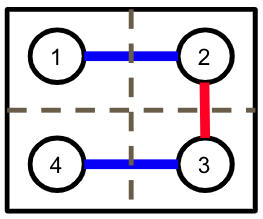
\includegraphics[width=0.25\textwidth]{Crest/Images/tinyGraph.png}}
    \qquad
    \subfloat[$RS\_Sols$]{\label{tab:solsTinyCity}
        \begin{tabular}[b]{c | c | c | c | c | c | c | c | c | c}
            \toprule
            VA & 0 & 1 & 2 & 3 & 4 & 5 & 6 & 7 & 8\\
            \midrule
            $C_1$ & 0 & 1 & 2 & 7 & 28 & 29 & 30 & 31 & 31\\
            $C_2$ & 0 & 22 & 26 & 27 & 28 & 29 & 30 & 30 & 30\\
            $C_3$ & 0 & 3 & 4 & 5 & 6 & 6 & 6 & 6 & 6\\
            $C_4$ & 0 & 1 & 27 & 29 & 30 & 31 & 32 & 32 & 32\\
            \bottomrule
        \end{tabular}
    }
    \qquad
    \subfloat[$NegVC\_Alloc$]{\label{tab:negVCTinyCity}
        \begin{tabular}[b]{c | c | c | c | c | c | c | c}
            \toprule
            Time & 0 & 1 & 2 & 3 & 4 & 5 & 6\\
            \midrule
            $C_1$ & 2 & 3 & 3 & 4 & 4 & 4 & 4\\
            $C_2$ & 2 & 1 & 2 & 1 & 2 & 2 & 2\\
            $C_3$ & 2 & 1 & 0 & 1 & 0 & 0 & 0\\
            $C_4$ & 2 & 3 & 3 & 2 & 2 & 2 & 2\\
            \hline
            $Exchange$ & - & 1-2 & 2-3 & 1-2 & 2-3 & - & -\\
                           &   & 3-4 &             & 3-4 &             &   &  \\
            \bottomrule
        \end{tabular}
    }
    \qquad
    \subfloat[$NegNumtrip petitionsSat$]{\label{tab:negNumtrip petitionsSatTinyCity}
        \begin{tabular}[b]{c | c | c | c | c | c | c | c}
            \toprule
            VA & 0 & 1 & 2 & 3 & 4 & 5 & 6\\
            \midrule
            $C_1$ & 2 & 7 & 7 & 28 & 28 & 28 & 28\\
            $C_2$ & 26 & 22 & 26 & 22 & 26 & 26 & 26\\
            $C_3$ & 4 & 3 & 0 & 3 & 0 & 0 & 0\\
            $C_4$ & 27 & 29 & 29 & 27 & 27 & 27 & 27\\
            \hline
            $OverallNumtrip petitionsSat$ & 59 & 61 & 62 & 80 & 81 & 81 & 81\\
            \bottomrule
        \end{tabular}
    }
    \caption{Vehicle Allocation Instance Example}
    \label{fig:myTinyCityFigure}
\end{figure}

The city has $numE \equiv 8$ AEVs to be allocated. A naive initial allocation evenly assigning 2 AEVs per SEC
is used (i.e., the initial $VC\_Alloc \equiv [2, 2, 2, 2]$). Figure \ref{fig:myTinyCityFigure}(c) shows how the number
of AEVs per SEC evolves over time as the
negotiation process progresses. For example, on time unit 1 a new column of the table is generated,
making $VC\_Alloc$ to evolve from $[2, 2, 2, 2]$ to $[3, 1, 1, 3]$.
The bottom row of the table highlights the negotiation steps leading to AEVs exchange on such time unit. (e.g., in time unit 1
both $(C_1, C_2)$ and $(C_3, C_4)$ agree to exchange AEVs among them). The amount of AEVs exchanged on each case can be
inferred by comparing consecutive rows of Figure \ref{fig:myTinyCityFigure}(c) (e.g., in time unit 0 $C_1$ and $C_2$
have 2 AEVs each, and in time unit 1 $C_1$ has 3 AEVs and $C_2$ has 1 EV, so they must have exchanged 1 EV).

A pair of SECs $c_i$ and $c_j$ decide on whether to exchange AEVs or not based on their local information;
they know both their current share in $VC\_Alloc$ (c.f. last column of Figure \ref{fig:myTinyCityFigure}(c))
and their respectives $RS\_Sols$ (c.f. Figure \ref{fig:myTinyCityFigure}(b)), which is a static table precomputed
in full before the negotiation process starts (c.f., Subsection \ref{ccis_and_smartgreens_relationship}).
However, the SECs $c_i$ and $c_j$ do not know the share
in $VC\_Alloc$ nor $RS\_Sols$ of any other SEC $c_z$ not involved in the negotiation.
For example, in time unit 1, when $C_1$ and $C_2$ start the negotiation with 2 AEVs each, they know they are currently
able to solve 2 and 26 TPs, resp. So, between them, 28 TPs. When they decide $C_1$ will borrow 1 AEVs from $C_2$,
they know this will lead to 7 and 22 TPs, resp. So, between them, 29 TPs, better than their current state. Similarly,
when $C_4$ borrows 1 AEVs from $C_3$, the two SECs pass from 31 TPs between them to 32 TPs.
Figure \ref{fig:myTinyCityFigure}(d)) shows how the number of TPs satisfied per SEC evolve over time, with its
last row measuring the $OverallNumtrip petitionsSat$, i.e., the quality of the current $VC\_Alloc$ (for example, in time unit 0
$OverallNumtrip petitionsSat$ is 59 TPs, but after the exchange of both ($C_1$, $C_2$) and ($C_3$, $C_4$) it reaches 61 TPs.

In the example the negotiation ends after 6 time units, as an entire negotiation cycle (steps 5 and 6) has happened
without a single EV exchange among connected SECs. During the negotiation process, $VC\_Alloc$ has evolved from
its initial $[2, 2, 2, 2]$ to $[4, 2, 0, 2]$ and the $OverallNumtrip petitionsSat$ from 59 TPs to 81 TPs.
The example confirms that a lightweight, pairwise strategy can converge rapidly to a
near‑optimal allocation, even with minimal initial information and only local decision‑making.

In this model, the SECs are assumed to behave as cooperative agents rather than strictly self-interested entities. Their negotiation decisions are guided by the collective goal of maximising the total number of TPs satisfied across the entire system. Although each SEC operates with local information—aware only of its own share in $VC\_Alloc$ and its precomputed $RS\_Sols$—the negotiation strategy is designed to promote exchanges that lead to global improvements.

For example, during a negotiation between $C_1$ and $C_2$ in time unit 1, both SECs assess whether reallocating an AEV results in a higher combined number of TPs satisfied. If this condition is met, the exchange proceeds, even if one SEC temporarily sacrifices resources. This cooperative approach reflects the underlying design of Smart Energy Communities, which aim to balance individual and collective benefits through resource sharing.

It is important to note that the model abstracts away from complex, self-interested behaviours or strategic deception, focusing instead on evaluating the performance of lightweight, decentralised, pairwise negotiations under cooperative assumptions. Future work could explore more adversarial or competitive negotiation dynamics.


\section{Reinforcement Learning-based Solution Approach}
\label{ccis_reinforcement_learning_solution_approach}

In this section, the chapter introduces a reinforcement learning-based solution as a decentralised approach to address the vehicle allocation problem \cite{Reference301} described in sections \ref{sec:ccis_problem}. 

\subsection{Deep Reinforcement Learning}
Deep Reinforcement Learning (DRL) trains agents to optimise cumulative rewards while making decisions \cite{Reference501}. Reinforcement learning and deep neural networks allow agents to learn complicated patterns and representations \cite{Reference501}.

\subsubsection{Q-Networks}
Q-networks are neural networks that approximate the Q-function, which estimates the expected cumulative reward an agent can obtain by taking a certain action from a given state and following a specific policy thereafter. The Q-network takes the current state as input and outputs Q-values for all possible actions, enabling the agent to make decisions that lead to higher rewards. The Q-value is calculated using the Bellman Equation \cite{Reference501}. 
\[
Q(s, a) = \sum_{s'} p(s' \mid s, a) \left[ r(s, a, s') + \gamma \max_{a'} Q(s', a') \right]
\]

Where:
\begin{align*}
Q(s, a) & : \text{Q-value for state-action pair }(s, a) \\
s & : \text{Current state} \\
a & : \text{Taken action in state } s \\
s' & : \text{Next state} \\
r(s, a, s') & : \text{Immediate reward obtained upon transitioning from state }  s\\ \text{ to state } s' \text{ with action } a \\
p(s' \mid s, a) & : \text{Transition probability to state } s' \text{ given action } a \text{ in state } s \\
\gamma & : \text{Discount factor that balances future rewards} \\
a' & : \text{Possible actions in state } s'
\end{align*}

% \subsubsection{Neural Networks}

% Neural networks are a class of machine learning models inspired by the structure and function of the human brain. They consist of interconnected nodes, called neurons, organised in layers. Each connection between neurons has associated weights that are learned during training. Neural networks can approximate complex functions and capture intricate relationships in data, making them suitable for tasks like function approximation, classification, and regression \cite{Reference502}.

\subsection{Problem Modeling}
In this formulation, each SEC acts as an independent agent that:

\begin{enumerate*}[label=(\roman*)]
    \item observes its local state (including available AEVs, pending TPs, and information from neighbouring SECs),
    \item selects an action (the fraction of AEVs to dispatch or retain),
    \item receives a reward balancing service quality and energy efficiency, and
    \item transitions to a new state, updating fleet distribution and trip queues.
\end{enumerate*}

The remainder of this subsection formally describes the Markov-game tuple \(M=(C, S, A, P, R, \gamma)\),where:

\begin{itemize}
    \item \(C\) is the set of agents, with each agent representing a SEC.
    \item \(S\) is the set of states, with each SEC maintaining its own state \(s_t^i\) at simulation step \(st\), incorporating the spatial distribution of available AEVs and TPs.
    \item \(A\) is the set of joint actions, allowing each agent to choose a fraction of available AEVs to dispatch to neighbouring SECs, represented as $a_t^i \in [0, 1]$. Each action $a_t^i \in A_i$ represents the fraction of available AEVs at SEC $c_i$ that will be dispatched to neighbouring SECs in the next simulation step $st+1$. For example, $a_t^i = 0.5$ means half of the available AEVs at SEC $c_i$ will be dispatched to neighboring SECs.
        \[ A_i = [0, 1] \]
    \item \(P\) represents the state transition probability which are deterministic. A $\epsilon$-greedy learning strategy, with a gradually decaying value of $\epsilon$ (exploration rate) is employed based on which an agent can choose to either take an action to explore the environment or an action that gains it the maximum reward based on its Q-network.
    \item \(R\) is the reward function that guides the decision making of the agents. It combines metrics such as petitions served and energy efficiency, as well as a shaping reward promoting efficient dispatching. It balances these factors through a weight parameter \(\alpha\)
        \begin{multline*}
            R_i(s_t, a_t^i) = \text{Petitions Served} - \\
            \alpha \cdot \text{Energy Usage of Dispatched AEVs}
            + R_{\text{shaping}}^i(s_t, a_t^i)
        \end{multline*}
        \begin{multline*}
                R_{\text{shaping}}^i(s_t, a_t^i) = -\alpha \cdot \text{Distance Covered by Dispatched AEVs} \\
                + \gamma \cdot \text{Petitions Served}
        \end{multline*}
    \item \(\gamma\) is the discount factor that determines the importance of future rewards.
\end{itemize}

\subsection{Instance Example}

For illustration purposes, a scenario involving three agents (SECs) denoted as \(A\), \(B\), and \(C\)is considered. The state of each agent at step \(st=0\) is represented by the number of available AEVs (\(EV_t^i\)) and the number of pending TPs (\(TP_t^i\)) in their respective service areas. The agents also select actions (\(a_t^i\)) by choosing a fraction of available AEVs to dispatch to neighbouring SECs. The reward function (\(R_i(s_t, a_t^i)\)) combines the number of petitions served, the energy usage of dispatched AEVs, and a shaping reward.

The following initial states and actions:

\begin{itemize}
    \item Agent \(A\): \(s_0^A = (8, 3)\) (8 available AEVs and 3 pending TPs)
    \item Agent \(B\): \(s_0^B = (5, 2)\) (5 available AEVs and 2 pending TPs)
    \item Agent \(C\): \(s_0^C = (7, 4)\) (7 available AEVs and 4 pending TPs)
\end{itemize}

The agents then choose actions for dispatching AEVs:

\begin{itemize}
    \item Agent \(A\): \(a_0^A = 0.6\) (60\% of available AEVs dispatched)
    \item Agent \(B\): \(a_0^B = 0.3\) (30\% of available AEVs dispatched)
    \item Agent \(C\): \(a_0^C = 0.4\) (40\% of available AEVs dispatched)
\end{itemize}

Assuming the following parameter values:
\begin{itemize}
    \item \(\alpha = 0.5\) (weight parameter for shaping reward)
    \item \(\gamma = 0.8\) (discount factor for shaping reward)
    \item Distance covered by each dispatched EV = 10 units
    \item Energy usage of each dispatched EV = 10 units
\end{itemize}

Based on these initial states, actions, and assumed parameter values, the shaping reward (\(R_{\text{shaping}}^i(s_t, a_t^i)\)) for each agent can be calculated:

\begin{itemize}
    \item Agent \(A\): 
    \[
    R_{\text{shaping}}^A(s_0^A, a_0^A) = -0.5 \cdot 10 + 0.8 \cdot 3 = -5 + 2.4 = -2.6
    \]
    \item Agent \(B\): 
    \[
    R_{\text{shaping}}^B(s_0^B, a_0^B) = -0.5 \cdot 10 + 0.8 \cdot 0 = -5 + 0 = -5
    \]
    \item Agent \(C\): 
    \[
    R_{\text{shaping}}^C(s_0^C, a_0^C) = -0.5 \cdot 10 + 0.8 \cdot 4 = -5 + 3.2 = -1.8
    \]
\end{itemize}

Finally, the total reward (\(R_i(s_t, a_t^i)\)) for each agent can be calculated by incorporating the shaping reward:

\begin{itemize}
    \item Agent \(A\): 
    \[
    R_A(s_0^A, a_0^A) = \text{Petitions Served} - 0.5 \cdot 10 - 2.6
    \]
    \item Agent \(B\): 
    \[
    R_B(s_0^B, a_0^B) = \text{Petitions Served} - 0.5 \cdot 3 - (-5) = \text{Petitions Served} - 0.5 \cdot 3 + 5
    \]
    \item Agent \(C\): 
    \[
    R_C(s_0^C, a_0^C) = \text{Petitions Served} - 0.5 \cdot 4 - (-1.8) = \text{Petitions Served} - 0.5 \cdot 4 + 1.8
    \]
\end{itemize}

The scenario example mentioned above represents a single step. In a reinforcement learning context, a complete sequence of actions, states, rewards, and transitions forms an episode. Each episode corresponds to a cycle of decision-making, action execution, state transitions, and rewards that occurs over a series of steps. The reinforcement learning algorithm learns from these episodes to develop an optimal policy that maximises cumulative rewards over time, adapting to the changing environment and interactions between agents.

\subsection{Decentralised DQN with Experience Sharing and GCN}
\label{sec:decentralised_dqn_gcn}

This subsection presents an enhanced decentralised DQN framework integrated with GCN \cite{Reference106}. The goal of this integration is to enable effective experience sharing and improve decision-making among SECs during the vehicle-allocation negotiation process.

% Learning Process Equations
Each SEC operates independently in its environment and interacts with the grid world. It selects an action based on an $\epsilon$-greedy policy using its own Q-network and exploration rate ($\epsilon$).

The SEC executes the action, receives a reward, and transitions to the next state. The experience tuple (state, action, reward, next\_state) is stored in the replay memory of the SEC.

The replay memory follows a First-In-First-Out (FIFO) mechanism, where old experiences are replaced with new experiences when the memory capacity is reached. The replay memory is used during the training process to sample random mini-batches of experiences. These mini-batches are then used to update the Q-network, allowing the agent to learn from a diverse set of experiences and improve its decision-making capabilities.

Mathematically, the replay memory can be defined as:
\[ D = \{(s, a, r, s')_1, (s, a, r, s')_2, \ldots, (s, a, r, s')_N\} \]

where $(s, a, r, s')_i$ represents the $i$-th experience stored in the memory. 

% Experience Sharing Equations and Diagram
Periodically, each SEC samples a random mini-batch of experiences from its replay memory $D$.

Now, to enhance the learning process and enable experience sharing between SECs, GCNs are introduced. A GCN performs iterative message passing between neighboring nodes (SECs) in the graph, enabling each SEC to incorporate information from its neighbors.

In the context of the grid world with SECs, each SEC corresponds to a node in the graph, and there are edges between spatially neighboring SECs. The features of each SEC (e.g., number of available AEVs, trips satisfied, energy consumed) form the node attributes.

The GCN aggregates information from neighboring SECs and updates the features and experience of the current community. This process enables the SEC to learn from the experiences of other SECs through the shared graph information.

Consider a simplified scenario with three SECs: communities A, B and C. These SECs are spatially connected in a grid-based system. Each SEC aims to optimise its energy allocation strategy to maximise the number of TPs served while minimising energy consumption.

Suppose we have the following features for each SEC:

\begin{itemize}
    \item SEC A: $\text{Num\_AEVs} = 50$, $\text{Num\_TPs} = 100$, $\text{Energy} = 700$
    \item SEC B: $\text{Num\_AEVs} = 30$, $\text{Num\_TPs} = 90$, $\text{Energy} = 600$
    \item SEC C: $\text{Num\_AEVs} = 40$, $\text{Num\_TPs} = 80$, $\text{Energy} = 400$
\end{itemize}

Initially, each SEC operates independently, using its own experience and Q-network to make decisions.

Imagine that SEC A wants to update its Q-values based on its experience and the experiences of its neighboring SECs (B and C). Through the GCN-based experience sharing mechanism, SEC A aggregates information from SECs B and C and updates its own features.

For example, suppose SEC A uses a simple message aggregation process where it takes an average of the features of its neighbors:

% \[
% \begin{aligned}
%     \text{New\_Num\_AEVs} &= \frac{\text{Num\_AEVs\_A} + \text{Num\_AEVs\_B} + \text{Num\_AEVs\_C}}{3} \\
%     % \text{New\_Num\_trip petitions} &= \frac{\text{Num\_trip petitions\_A} + \text{Num\_trip petitions\_B} + \text{Num\_trip petitions\_C}}{3} \\
%     % \text{New\_Energy} &= \frac{\text{Energy\_A} + \text{Energy\_B} + \text{Energy\_C}}{3}
% \end{aligned}
% \]
\[
\text{New\_Num\_AEVs} = \frac{1}{3} \sum_{i=A}^{C} \text{Num\_AEVs\_i}
\]


This averaging process integrates information from neighboring SECs. After the aggregation, the new features for SEC A become:
\begin{itemize}
    \item $\text{New\_Num\_AEVs} = 40$
    \item $\text{New\_Num\_TPs} = 90$
    \item $\text{New\_Energy} = 566.67$
\end{itemize}

Now, SEC A can use these updated features in its Q-network to make more informed decisions. By considering information from neighboring SECs, SEC A can learn from their experiences, understand the overall energy allocation dynamics in the network, and adjust its EV allocation strategy. 

\subsection{Algorithm Overview}
This subsection describes of the proposed Decentralised DQN-GCN algorithm through pseudocode. Specifically, Algorithm 2 illustrates how messages (or experiences) are shared among neighbouring SECs using a GCN. Each SEC (node \( v_i \) in graph \( \mathcal{G} \)) aggregates relevant information from its neighbours to enhance its own learning and decision-making process. The function \(\text{Neighbors}(v_i)\) identifies neighbouring SECs directly connected to \( v_i \), enabling each community to learn not only from its own experiences but also from the experiences of its peers.


% Algorithm \ref{algo:gcn} presents the pseudocode for message passing. It assumes that $\text{Neighbors}(v_i)$ is a function that returns the set of neighboring nodes of $v_i$ in the graph $\mathcal{G}$. 

The learning process involves a series of steps that enable each SEC to operate effectively within the ride-sharing environment, making informed decisions through the integration of GCNs for experience sharing and learning. A three-layer GCN was adopted to capture both immediate and second-order neighbourhood information without introducing excessive depth that could cause over-smoothing or vanishing gradients. The number of neurons per layer is set to match the number of SECs in the system, ensuring a direct, interpretable mapping between graph nodes and learned representations. The ReLU activation function and a learning rate of $\alpha = 0.001$ were chosen following preliminary tuning experiments, balancing training stability and learning speed.

These parameter choices reflect a trade-off between model complexity and the practical requirements of operating on dynamic, city-scale graphs representing SEC interactions.
\begin{algorithm}[hb]
\caption{Message Passing in GCN for Decentralised Deep Q-Learning with GCN Experience Sharing}
\small % Adjust font size
\SetAlgoLined
\SetKwInOut{Input}{Input}
\SetKwInOut{Output}{Output}

\Input{Graph $\mathcal{G}$ for each SEC, GCN architecture parameters, GCN hyperparameters}
\Output{Updated graph representation for each SEC}

\ForEach{SEC in SECs}{
    \textbf{Initialize} node embeddings $\mathbf{H}$ for each node in $\mathcal{G}$ with random values\;
}

\ForEach{layer in GCN layers}{
    \ForEach{SEC in SECs}{
        \textbf{Initialize} message aggregator $\mathbf{M}_v$ for each node $v$ in $\mathcal{G}$ with zeros\;
        
        \ForEach{node $u$ with an edge to $v$}{
            \textbf{Aggregate} messages from neighbors: $\mathbf{M}_v \pluseq \text{Aggregator}(\mathbf{H}_u)$\;
        }
        
        \textbf{Update} node embeddings using GCN layer: $\mathbf{H}_v \pluseq \text{GCNLayer}(\mathbf{H}_v, \mathbf{M}_v)$\;
    }
}
\textbf{Return} updated node embeddings $\mathbf{H}$ for each SEC\;
\end{algorithm} \label{algo:gcn}

\begin{itemize}
    \item \textbf{GCN Parameters:} Configuration settings that define the structure and behavior of the GCN. These parameters include the number of layers, the number of neurons in each layer as presented in Table \ref{tab:gcn_table}.

    \item \textbf{Node Embeddings:} Vectors that represent the features of each node (SEC) in the graph. These embeddings capture important information such as the number of available AEVs, trips served, and energy consumption for each SEC.
\end{itemize}
\begin{algorithm}[ht]
\caption{Decentralised Deep Q-Learning with GCN Experience Sharing for DeepTripsEnvironment}
\small % Adjust font size
\SetAlgoLined

\SetKwInOut{Output}{Output}

\Output{Optimal Q-networks for each SEC}

\textbf{Initialize} replay memory $D$ with maximum capacity $N$\;
\textbf{Initialize} Q-networks $Q$ for each SEC with random weights\;
\textbf{Initialize} target networks $Q_{\text{target}}$ for each SEC with the same weights as $Q$\;
\textbf{Initialize} total number of episodes $N$\;

Set learning rate $\alpha$, discount factor $\gamma$, exploration rate $\epsilon$, and GCN parameters\;

\textbf{Initialize} GCN for each SEC with random weights\;

\For{$episode \gets 1$ to $N$}{
    \textbf{Reset} environment to initial state\;
    
    \ForEach{SEC in SECs}{
        \textbf{Reset} SEC-specific parameters (vehicles, trips)\;
    }
    
    \While{not reached the terminal state}{
        \ForEach{SEC in SECs}{
            \textbf{Observe} current state $s$ for the SEC\;
            
            \textbf{Obtain} graph representation for the SEC using GCN\;
            
            \textbf{Choose} action $a$ using $\epsilon$-greedy policy based on $Q$ for the SEC\;
            \textbf{Execute} action $a$ for the SEC and \textbf{observe} reward $r$ and next state $s'$\;
            
            \textbf{Store} experience $(s, a, r, s')$ in replay memory $D$ for the SEC\;
        }
        
        \ForEach{SEC in SECs}{
            \textbf{Sample} random mini-batch of experiences from $D$ for the SEC\;
            
            \ForEach{experience in mini-batch for the SEC}{
                \textbf{Obtain} graph representation for the SEC using GCN\;
                
                \textbf{Update} target values using target network $Q_{\text{target}}$ for the SEC\;
                
                \textbf{Update} Q value for $(s, a)$ using reward function %(see Section \ref{sec:problem_instance})\;
            }
        }
        
        \textbf{Update} current state $s$ to next state $s'$ for each SEC\;
    }
    
    \ForEach{SEC in SECs}{
        \textbf{Update} target network $Q_{\text{target}}$ with weights from $Q$ for the SEC\;
    }
    
    \textbf{Decrease} $\epsilon$ (exploration rate) over time\;
}
\end{algorithm} \label{algo:decentralised_vehicle_allocation}

\begin{table}[h]
    \centering
    \caption{GCN Parameters, Layers, and Neurons}
    \begin{tabular}{@{}lll@{}}
    \toprule
    \textbf{Parameter} & \textbf{Description} & \textbf{Value} \\ \midrule
    \textbf{Number of Layers} & Depth of GCN architecture & 3 \\
    \textbf{Number of Neurons per Layer} & Dimensionality of representations & SECs  \\
    \textbf{Activation Function} & Non-linear activation & ReLU \\
    \textbf{Learning Rate \(\alpha\)} & Gradient descent step size & 0.001 \\ \bottomrule
    \end{tabular}
    \label{tab:gcn_table}
\end{table}

\section{Evaluation}
\label{sec:evaluation}

Subsection \ref{sec:experimental_setup} describes the alignment of existing benchmarks (i.e. Google HashCode) and public
datasets (i.e. NYC taxis) to the proposed problem formulation, specifically enabling the evaluation over different
SEC connectivity levels transport request distributions.
Then, Subsection \ref{analysis_performance_scalability} discusses the performance and scalability of the RL
solution approach.

\subsection{Experimental Setup}
\label{sec:experimental_setup}

A Google HashCode'18 \emph{GHC\_base\_instance} (namely \emph{metropolis.in}) and a New York City dataset  \emph{NYC\_base\_instance}
(with a fraction of 1 day taxi trips in NYC)
are selected. From now on they are referred to as \emph{GHC\_i} and \emph{NYC\_i}, resp.
Both base instances are then aligned to the proposed vehicle allocation and ride-sharing problem tandem, by including
$numC$ SECs spread across the city,
$numE$ vehicles with a given battery and passenger capacities ($e_{bc}$ and $e_{pc}$) and
the set of neighbour transport requests TPs of each SEC. The resulting instances are referred to as
\emph{GHC\_ai} and \emph{NYC\_ai}, resp.

Specifically, \emph{GHC\_ai} contains 16 SECs, 400 AEVs and overall 10,000 TPs;
\emph{NYC\_ai} contains 256 SECs, 1,536 AEVs and overall 50,000 TPs.

These aligned base instances were respectively used as the seed for
generating the \emph{GHC\_aligned\_benchmark} and the \emph{NYC\_aligned\_benchmark}
(fron now on \emph{GHC\_ab} and \emph{NYC\_ab}), each of them containing a
set of instances with a number of SEC-connections ranging $[(numC - 1), \ldots, (numC * (numC + 1))/2]$.
The smallest instance (i.e., the one containing $numC - 1$ connections) represents a scenario with a
connection between each pair of consecutive SECs $c_i$
and $c_{i+1}$. The largest instance (i.e., the one containing $(numC * (numC + 1))/2$ connections) represents a scenario
where each pair of SECs $c_i$ and $c_j$ are connected.
The instances of the benchmark are generated incrementally, from smallest to largest,
with each new $instance_{i+1}$ reusing all connections from $instance_{i}$, and adding a novel SEC connection
($c_i$, $c_j$) not included in $instance_{i}$.

Specifically, \emph{GHC\_ab} contains 106 instances, with the number of connections ranging from 15 to 120. For \emph{NYC\_ab}, due to the extensive range of potential connections (from 255 to 32,640), a representative subset of 38 instances was systematically selected. The selection involved evenly sampling connection counts across the entire range, ensuring instances represented the spectrum from minimally connected to highly connected scenarios. Specifically, instances with the following numbers of connections were chosen:  
\[255, 330, 500, 1000, 1500, 2000, 2500, 3000, 3500, 4000, 4500, 5000, 5500, 6000, 6500,\]
\[7000, 7500, 8000, 8500, 9000, 9500, 10000, 12000, 14000, 16000, 18000, 20000, 22000,\] 
\[24000, 26000, 28000, 30000, 31000, 31500, 31800, 32000, 32200, 32640.\]

Finally, to evaluate the impact of the transport request distribution on the performance of the solution approach,
variants of the \emph{GHC\_ab} and \emph{NYC\_ab} are generated by modifying the mapping of TPs to SECs.
Specifically, a constant distribution, with all SECs receiving the same number of TPs, is tried first, namely
\emph{GHC\_abc} and \emph{NYC\_abc}.
Then, a set of normal distributions, with sigma values ranging
in $[0.5, 1.5, \ldots, 4.5]$ (thus varying the number and extent of differences in the TPs of each SEC) are tried,
namely \emph{GHC\_abn\_0.5}, \emph{NYC\_abn\_0.5} and so on.

In all cases, when solving an instance, the vehicle allocation problem is solved using the Decentralised RL solution
approach based on Deep Q-Learning with GCN Experience Sharing (c.f., Section \ref{ccis_reinforcement_learning_solution_approach}).
100 episodes were used, with a gradually decaying value of the exploration rate $\epsilon$ to $0.1$ over the episodes.
As per the underlying ride-sharing problem of each SEC, $RS\_Sols$ is precomputed using the reactive-based
simulation on top of a greedy decision-making process (c.f., Chapter \ref{chapter3}).
Experiments are carried out on a computer with a AMD Ryzen 7 3800X 8-Core Processor (3.89 GHz), 64GB RAM,
1TB SSD, and NVIDIA GeForce RTX 2080 Super.

\subsection{Analysis - Performance and Scalability}
\label{analysis_performance_scalability}
As described in Section \ref{ccis_and_smartgreens_relationship}, the
quality of a solution is measured as the overall number of TPs serviced among all SECs $OverallNumtrip petitionsSat$
(from now on $qr$, for quality result).

On the one hand, the optimal solution of \emph{GHC\_ai} and \emph{NYC\_ai}
is computed
using the MIP-based centralised formulation presented in Section \ref{ccis_centralised_formulation}.
From now on, this value is referred to as $qr\_ub$, for upper-bound on the quality result.
Specifically, for \emph{GHC\_ai} $qr\_ub$ is 5,196 TPs; for \emph{NYC\_ai}
$qr\_ub$ is 35,724 TPs.

On the other hand, a lower bound $qr\_lb$ for \emph{GHC\_ai} and \emph{NYC\_ai} is computed by
evenly distributing the vehicles among the SECs.
Specifically, for \emph{GHC\_ai}
this means 25 AEVs per each of the 16 SECs, a vehicle allocation leading to $qr\_lb$ of 4,679 TPs;
for \emph{NYC\_ai}
this means 6 AEVs per each of the 256 SECs, a vehicle allocation leading to $qr\_lb$ of 34,091 TPs.

The range $[qr\_lb, \ldots, qr\_ub]$ represents the window of opportunity for each instance to improve its $qr$.
Specifically, each instance
of \emph{GHC\_abc}, \emph{GHC\_abn}, \emph{NYC\_abc}, \emph{NYC\_abn}
is set to start the negotiation process with the naive vehicle distribution (and thus having an initial $qr$
equal to $qr\_lb$).
Then, the final solution $qr$ found by the instance (after completing its negotiation process) is measured by
%positioning it on
its percentile in the range
$[qr\_lb, \ldots, qr\_ub]$ (i.e., the closer the percentile is to 100\%, the closer the solution found by the instance
$qr$ is to the optimal solution $qr\_ub$).

Figure \ref{fig:resultsFigure} presents the results of the experiments.
\begin{figure}[htbp]
    \centering
    \subfloat[Percentile of \emph{GHC\_abc}]{\label{fig:tinyCity}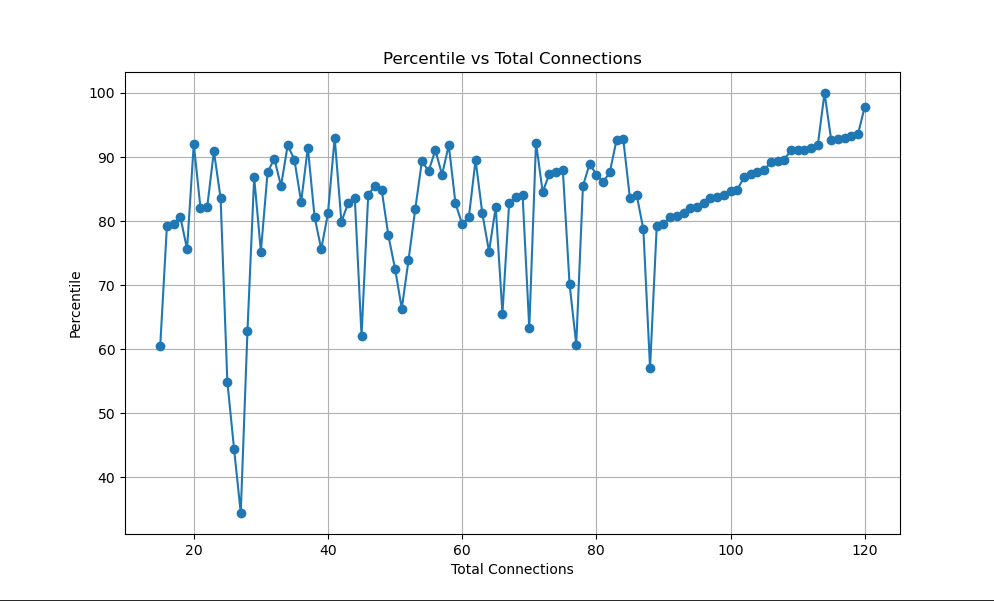
\includegraphics[width=0.75\textwidth]{Crest/Images/percentile_ghc.png}}
    \qquad
    \subfloat[Percentile of \emph{NYC\_abc}]{\label{fig:tinyCity}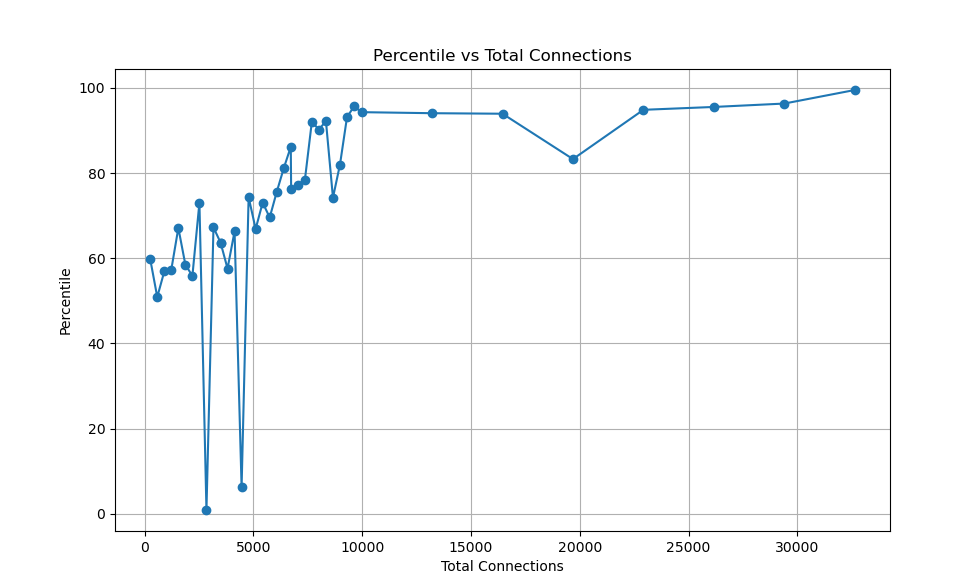
\includegraphics[width=0.75\textwidth]{Crest/Images/percentile_nyc.png}}
    \qquad
    \subfloat[Multi-objective Results for \emph{GHC\_abc}]{\label{fig:tinyCity}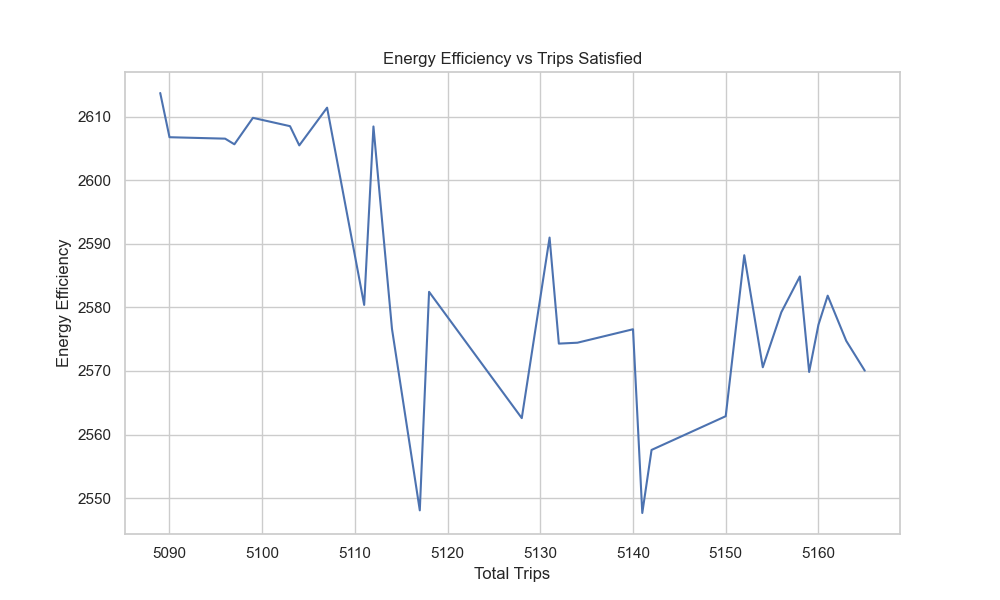
\includegraphics[width=0.75\textwidth]{Crest/Images/metropolis_energy_consumption_converge.png}}
    \caption{Performance Results}
    \label{fig:resultsFigure}
\end{figure}
Specifically, Figure \ref{fig:resultsFigure}(a) (resp. Figure \ref{fig:resultsFigure}(b)) presents the percentile of the
solution $qr$ when solving the instances of \emph{GHC\_abc} (resp. \emph{NYC\_abc}); results for the normal
distributions are omitted, as they are quite similar to the displayed ones.
The decentralised negotiation process carried out by the RL solution approach proves to find high quality solutions,
with $qr$ in a percentile of 60+ for all instances.
Moreover, it seems to be a trend that the higher the number of connections among SECs, the higher the $qr$
obtained, being able to find near optimal solutions when almost all connections are enabled.
A few outlier configurations are observed, with a temporary reduction in the increasing trend of $qr$.
This can be attributed to the $\epsilon$-greedy learning process. The SECs explore the environment to learn optimal policies that maximise the
expected rewards, which might lead to consecutive suboptimal actions that are hard to recover from afterwards.

As the total number of connections between SECs increases, two key trends emerge:

\begin{enumerate}
    \item \textbf{Improved Performance:} With more inter-SEC connections, the network becomes more flexible, providing additional pathways for vehicle exchanges. This structural redundancy allows the decentralised Q-Learning algorithm to better reallocate AEVs, resulting in solutions that converge closer to the centralised MILP-derived upper bound. In essence, increased connectivity reduces geographic or resource isolation, enabling SECs to balance their vehicle availability more effectively.

    \item \textbf{Reduced Variability:} The observed reduction in result variability as connections increase is attributed to the diminishing influence of initial allocation imbalances or specific network topologies. Sparse networks are more sensitive to initial conditions or local constraints, which can lead to higher solution variability. In contrast, well-connected networks offer more consistent reallocation opportunities across all SECs, stabilising performance outcomes.
\end{enumerate}

These findings align with general principles in network optimisation and multi-agent systems, where enhanced connectivity improves resource flow and system robustness, particularly under decentralised decision-making frameworks \cite{klapp2020decentralized}.

In terms of the multi-objective goal of the RL solution approach
(i.e., the number of TPs serviced vs the energy consumption of the AEVs)
Figure \ref{fig:resultsFigure}(c) indicates that the reward function contributes to a more stable energy consumption pattern as the number of connections among SECs increase.
This indicates that SECs with shorter average journey durations are favoured over those with longer travels, leading to enhanced energy efficiency.  Nonetheless, this prioritising necessitates meticulous evaluation.  Focussing on shorter travels can improve overall system efficiency by decreasing energy consumption per trip, but it may unintentionally harm groups whose mobility requirements naturally entail greater distances.  A balanced approach is essential: the system must pursue overall efficiency while maintaining service fairness among localities.  Future research should investigate strategies to dynamically modify this priority, taking into account both energy efficiency and equitable access to mobility services.
 %However, it is important to note that this value
%may further increase once more sophisticated vehicle-passenger routing algorithms are incorporated.

Finally, in terms of scalability, the RL solution approach
is able to solve each instance of each of the benchmarks in less than 15 seconds, with an average execution time
per instance of 10.57 seconds. This indicates that the
proposed approach is efficient and capable of handling very large instances (with thousands of trips and vehicles),
potentially making it suitable for its application to real-world scenarios.

\section{Effect of EV Fleet Size on Performance}
\label{sec:fleet_size_performance}
This section explores how varying the number of autonomous electric vehicles (AEVs) allocated to the system influences overall performance, particularly focusing on trip satisfaction and energy efficiency.

\subsection{Objective}
This section evaluates the impact the size of the AEV fleet has in terms of number of TPs being served and energy consumption. 

\subsection{Experimental Setup}
To study the impact of fleet size, the number of AEVs in the city are kept at 50\%, 100\%, and 150\% of the ones of the instances (\emph{GHC\_ai})(i.e., 200, 400 and 600 AEVs, respectively). 

The performance of the system is evaluated in terms of two primary metrics:
\begin{itemize}
    \item \textbf{Number of trips served}: The total number of TPs successfully allocated and served during the simulation.
    \item \textbf{Energy consumption}: The total energy consumed by the fleet to serve the trips.
\end{itemize}

Each configuration employs the RL-based solution approach, which involves 100 episodes. Each experiment used the identical hardware specified in Section \ref{sec:experimental_setup}.

% \subsection{Expected Outcome}
% The experiment is expected to provide insight into the impact of fleet size on the quality of the ride-sharing solution and the system's energy efficiency. Increasing the number of AEVs should initially result in more trips being served, but diminishing returns are expected after reaching a certain fleet size. This could indicate the optimal fleet size for the given city configuration.

\subsection{Results and Analysis}
Table \ref{tab:fleet_size_results} shows the results of the experiments, comparing the number of trips served and energy consumption across different fleet sizes. Figure \ref{fig:fleet_size_performance} shows a visual comparison of the outcomes.


\begin{table}[htbp]
    \centering
    \caption{Effect of EV Fleet Size on Performance}
    \label{tab:fleet_size_results}
    \begin{tabular}{|c|c|c|c|}
        \hline
        \textbf{Fleet} & \textbf{TP Served} & \textbf{Energy(units))} & \textbf{Energy Efficiency (TP/units)} \\
        \hline
        50\% Fleet  & 4,200 & 12,500 & 0.336 \\
        100\% Fleet  & 5,196 & 15,000 & 0.346 \\
        150\% Fleet & 5,250 & 17,500 & 0.300 \\
        \hline
    \end{tabular}
\end{table}

Table \ref{tab:fleet_size_results} show that, as the fleet size increases, so it does the number of TPs being served. However, in terms of energy efficiency, a peak is reached by the medium-sized AEVs fleet, for it to decrease when moving to the high-sized AEVs fleet.

This indicates that, while growing the fleet size enables for more trips to be served, the system eventually reaches a threshold of diminishing returns, at which adding more vehicles results is a less efficient use of energy.

\begin{figure}[htbp]
    \centering
    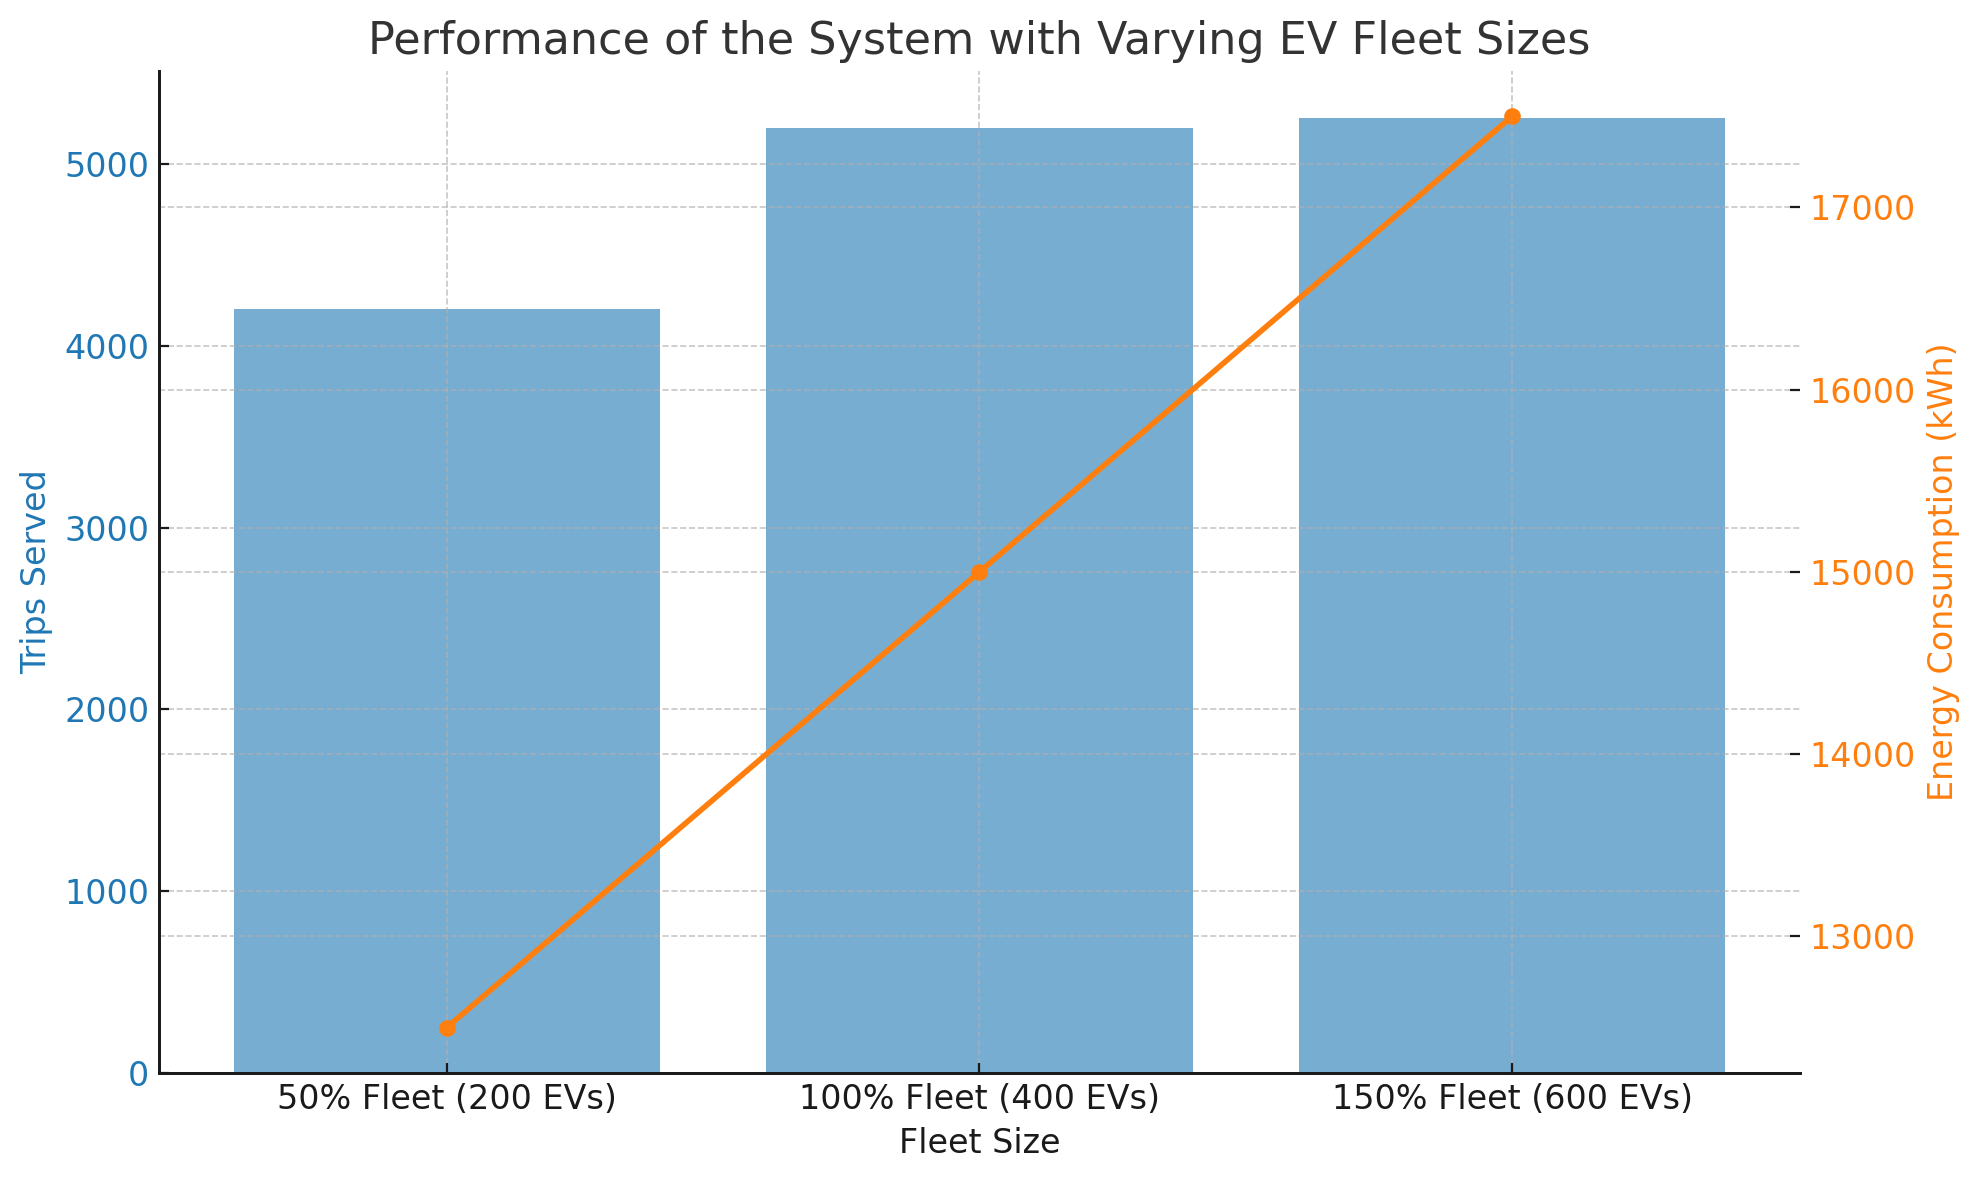
\includegraphics[width=0.75\textwidth]{Crest/Images/fleet_size_performance.png}
    \caption{Performance of the system with varying EV fleet sizes}
    \label{fig:fleet_size_performance}
\end{figure}


% \subsection{Conclusion}
The experimental results show that increasing the number of AEVs improves the total number of trips served, but only to a degree. Beyond this limit, the energy efficiency of the system declines. Further increases in fleet size result in declining returns and lower energy efficiency, which should be considered when scaling up EV fleets in real-world scenarios.

\section{Conclusions}
\label{sec:conclusion}

This chapter has presented the design, implementation and evaluation of the vehicle fleet allocation in a SEC-based
ride-sharing service, proposing a decentralised alternative
to the traditional central management in rapidly growing cities
(which are prone to dynamic urban environments and fluctuating travel demands).
On it, the independent SECs of the city compete for the allocation of AEVs resources,
which then they use to operate the TPs of its own neighbours via ride-sharing.
The vehicle allocation
problem has been formulated as a decentralised, iterative negotiation process among independent SECs,
where connected SECs decide the potential exchange of AEVs among them, based solely on their local information.
The underlying ride-sharing service operated by each SEC has been formulated using the ride-sharing model proposed in Chapter 3.
A solution approach to the problem tandem has been presented, using a Multi-Objective and Multi-Agent
RL algorithm, involving Deep Q-Learning with Graph Convolutional Networks, for SECs to
learn from previous negotiations.
The solution approach has been tested by aligning existing benchmarks (i.e. Google HashCode) and public
datasets (i.e. NYC taxis) to the proposed problem formulation, evaluating different SEC connectivity-levels
and transport request distributions.
The RL algorithm has proven to output high quality solutions in all cases, providing even near optimal solutions
when almost all SECs are able to exchange vehicles. Moreover, the RL algorithm has proven to scale well,
handling very large instances (with thousands of trips and vehicles) in just a few seconds, and therefore
potentially making it suitable for its application to real-world urban transportation systems. The complete code can be accessed via GitHub \cite{chapter4code}.

% The proposed approach provides multiple opportunities for future work.
% On the one hand, incorporating adaptive learning rates into the training procedure so that the model can adapt and fine-tune its parameters based on the current state of the system will be investigated to increase the overall learning efficacy.
% On the other hand, the ride-sharing service can be integrated with real-time traffic conditions, user preferences, and other dynamic variables, as well as the use of a dynamic charging infrastructure (consisting of both fixed and mobile charging stations), in order to promote more sustainable urban mobility.